\chapter{Introducción específica} % Main chapter title

\label{Chapter2}

%----------------------------------------------------------------------------------------
%	SECTION 1
%----------------------------------------------------------------------------------------
Durante este capítulo se brinda un marco orientativo sobre los requerimientos específicos del proyecto, la teoría básica involucrada y las tecnologías utilizadas para su realización.

\section{Requerimientos}
El trabajo realizado es un equipo adquisidor de DP que tiene como cliente a la UTN FRGP. 

A continuación se listan los requerimientos acordados al iniciar el trabajo. Cabe destacar que todos fueron cumplimentados en su totalidad con excepción de los requerimientos 23 y 24 que fueron modificados, de mutuo acuerdo con el cliente, sin generar deterioro alguno en las características del equipo.

\begin{enumerate}[label=\textbf{Req \arabic*}]
\item el dispositivo deberá, mediante el procesamiento de las adquisiciones, detectar los picos máximos de los pulsos de DP y representarlos sobre una senoide de referencia de frecuencia industrial - 50 Hertz - en fase con la tensión de ensayo (generar un patrón de DP).
\item el dispositivo deberá funcionar como un sistema \textit{stand-alone}.
\item el dispositivo deberá mantener la fecha y hora por medio de un RTC.
\item el dispositivo deberá tener un puerto de acceso serial (preferentemente diferencial) para configuración y acceso a datos remoto.
\item el dispositivo deberá contar con un puerto USB para la descarga de los patrones de DP.
\item el dispositivo deberá permitir modificar el umbral de disparo a partir del cual se comenzará a adquirir una señal.
\item el dispositivo deberá permitir modificar la cantidad de muestras que serán adquiridas por disparo (máximo 1000).
\item el dispositivo deberá permitir modificar la cantidad de disparos (máximo 1000) que componen a un patrón de DP.
\item el dispositivo deberá permitir configurar el RTC.
\item el dispositivo deberá permitir planificar la generación automática de un patrón DP cada periodos múltiplos de 1 hora (calendario).
\item el dispositivo deberá permitir generar un patrón de DP con los parámetros configurados a demanda y transferirlo por el puerto serie.
\item el dispositivo deberá permitir poner al sistema en modo “ARMADO” o “ DESARMADO”.
\item en modo “ARMADO” el dispositivo deberá cumplir con las adquisiciones preestablecidas por calendario.
\item en modo “DESARMADO” el dispositivo no estará operativo.
\item la entrada de señal de referencia debe poder detectar los cruces por cero de una senoide de 50 Hz, y saber su polaridad.
\item la entrada de señal de referencia debe ser opto-acoplada.
\item el dispositivo deberá llevar un contador en milisegundos a partir de la señal de cruce por cero. De forma tal que se pueda saber en todo momento si está transcurriendo un semiciclo positivo o negativo y saber cuánto tiempo transcurrió desde su inicio.
\item se deben poder adquirir señales con una ancho de banda entre 0.1 MHz y 40 MHz con una resolución mínima de 8 bits.
\item la amplitud máxima de la señal de entrada será de 1 Vpp.
\item la entrada para el sensor analógico deberá ser de 50 ohms diferencial.
\item el dispositivo deberá detectar cuando la señal muestreada supere el umbral de disparo, si esto sucediera las siguientes muestras (cantidad definida anteriormente en la configuración) deberán ser comparadas entre sí y preservar la de mayor magnitud. El valor obtenido deberá ser almacenado en memoria, junto con un timestamp, la polaridad del semiciclo de referencia y su momento angular. Este proceso debe ser repetido hasta que se cumplan los disparos que componen un patrón DP.
\item deberá indicará su estado “ARMADO - DESARMADO” por medio de un led de estado.
\item \label{req:23}deberá permitir “ARMAR - DESARMAR” al sistema por medio de una tecla física.
\item \label{req:24}deberá realizar la acción de transferir a un pendrive el contenido total de la memoria interna por medio de una tecla fısica.
\item el dispositivo deberá listar todos los patrones de DP almacenados bajo el siguiente identificador “AAMMDDhhmm” en base a la fecha de generación del patrón.
\item el dispositivo deberá permitir seleccionar al patrón por medio de su identificador y solicitar su transferencia por puerto serie.
\end{enumerate}

Los requerimientos 23 y 24 fueron modificados debido a que el almacenamiento de las DP es realizado directamente en el pendrive. De esta forma se puede reducir el costo en el diseño y se elimina la necesidad de transferir archivos entre memorias. Ambos requerimientos fueron reemplazados por el siguiente:
\begin{itemize}
\item deberá almacenar en el pendrive el patrón de DP al finalizar su adquisición.
\end{itemize}


\section{Descripción general del sistema}

En la figura \ref{fig:bloques} se brinda una introducción de los módulos principales que abarcan el sistema y su interacción, por medio de esta se busca brindar una mejor interpretación de algunos temas abordados en este capítulo.

\begin{figure}[ht]
	\centering
	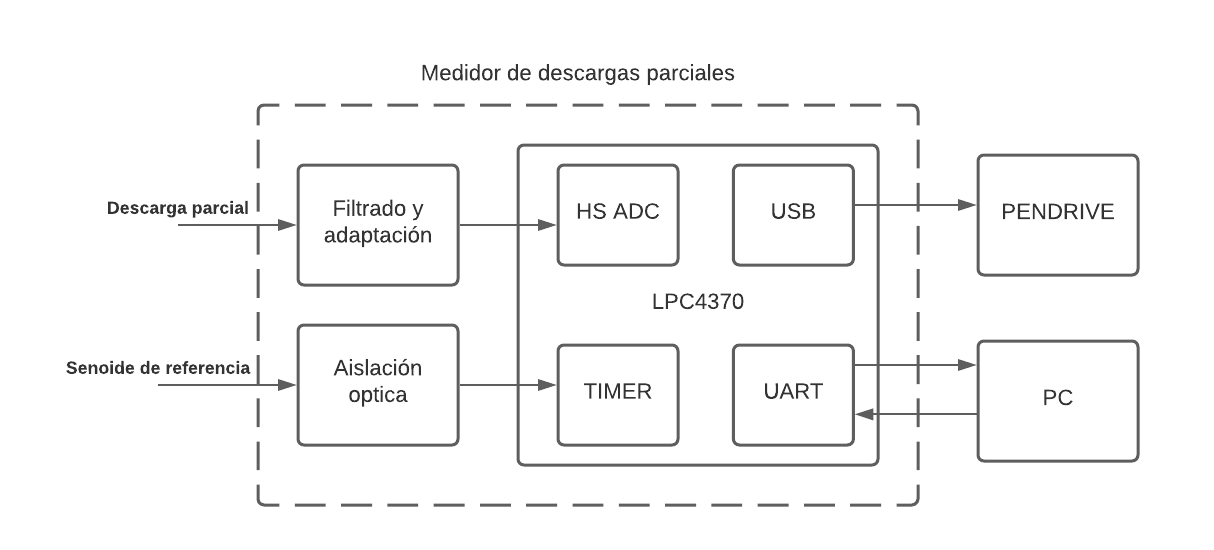
\includegraphics[width=\textwidth]{./Figures/bloques.png}
	\caption{Diagrama en bloques de sistema.}
	\label{fig:bloques}
\end{figure}

El objetivo principal del equipo consiste en adquirir, almacenar y procesar señales de DPs para posteriormente, junto a la senoide de referencia, conformar el diagrama de magnitud-fase o patrón de DP.

\section{Aislación óptica}
Un optoacoplador es un dispositivo que vincula de forma óptica un diodo led y un fototransistor a través  de material aislante transparente. Utilizados como interfaz entre circuitos con diferentes potenciales de masa, los optoacopladores reemplazan la aislación por medio de transformadores y relés. También son utilizados para aislar circuitos lógicos y líneas de potencia evitando cambios de impedancia, mejorando la capacidad de aislación entre entrada y salida y facilitando la eliminación del ruido \citep{opto:appnote}. Para este equipo se seleccionó el optoacoplador LTV357 \citep{opto:ltv357} de la empresa liteon, el mismo cumple con los requisitos de ser de bajo costo, tener una aislación de 3750 Vrms y una respuesta lineal hasta 2 KHz de frecuencia.

\begin{figure}[ht]
	\centering
	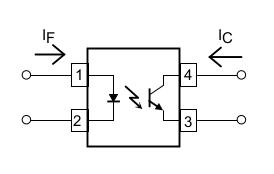
\includegraphics[width=70mm]{./Figures/opto.png}
	\caption{Representación esquemática de un optoacoplador.}
	\label{fig:opto}
\end{figure}

\section{Filtrado y adaptación}
Una etapa de filtrado y adaptación es un punto crítico para cualquier diseño de adquisición de señales analógicas. La señal proveniente de los sensores puede contener componentes de frecuencia fuera del ancho de banda de interés. También es posible que los niveles de tensión de la señal no utilicen al máximo el rango dinámico de entrada perdiendo bits de conversión. La saturación por sobretensión también es un elemento que perjudica a la calidad de las mediciones y en algunos casos puede destruir al equipo. 

La etapa de filtrado está diseñada para dejar pasar las frecuencias dentro de la banda de interés, atenuando en gran parte a todas aquellas fuera de rango.

La etapa de adaptación permite llevar los niveles de tensión de entrada al máximo rango dinámico permitido, esto puede realizarse por medio de amplificación o atenuación de la señal dependiendo el caso. En esta etapa también se implementan protecciones por sobretensión que puedan dañar al equipo, normalmente diseñadas con diodos de alta velocidad.

\section{Procesamiento}
La etapa de procesamiento es la encargada de orquestar todos los módulos del sistema. El equipo utiliza como microcontrolador principal un LPC4370 \citep{micro:lpc4370} de la firma NXP. La elección fue determinada porque posee un conversor analógico digital de alta velocidad (80 MSPS) combinado con un procesador ARM cortex M4 y dos ARM cortex M0. También incluye en la versión con encapsulado TFBGA100 dos periféricos USB de alta velocidad, puerto serie, reloj de tiempo real y entradas de propósito general.

Fue determinante para su elección el periférico ADCHS y su bajo costo. Gracias a que los principales módulos del desarrollo pudieron ser resueltos con los periféricos internos, solo fue necesario implementar de forma externa la etapa de aislación óptica y la etapa de adaptación y filtrado de señal.

Periféricos utilizados: 
\begin{itemize}

\item HS ADC - Conversor analógico digital de alta velocidad

El LPC4370 TFBGA100 dispone de 3 conversores analógicos digitales de alta velocidad. Este es un periférico complejo que permite realizar adquisiciones analógicas a una tasa de muestreo de 80 MSPS con una resolución de 12 bits. Para poder manejar este flujo de datos proporciona conexión por DMA. Otro característica importante es el sistema de disparo del trigger, que permite dos umbrales de disparo por flanco ascendente o descendente.

\item Timers

Dispone de 4 timers de 32 bits, que permiten ser configurados como contadores o temporizadores. Para permitir una mejor adaptación a los tiempos de aplicación, proporcionan divisores y diferentes opciones suministro de clock.


\item USB

Dispone de 2 puertos USB 2.0 con velocidad de transferencia de hasta 480 Mb/s. Uno de ellos con tecnología on-the-go. Ambos soportan DMA  y cumplen con las especificaciones Universal Serial Bus 2.0

\item RTC - Reloj de tiempo real

Dispone de un reloj de tiempo real con registros específicos para funcionar en bajo consumo. Este módulo requiere de un cristal propio de 32 KHz para generar una base de tiempo de 1 Hz independiente al CPU, también posee una línea de alimentación dedicada que puede ser alimentada por batería.
\end{itemize}


\section{Muestreo de datos}
Para procesar y almacenar las señales analógicas de alta frecuencia proveniente del pulso de una DP es preciso realizar un muestreo de amplitud de la señal. 

El concepto de muestreo de amplitud de una señal analógica en intervalos de tiempo discretos se muestra en la figura \ref{fig:muestreo1}.

La señal analógica debe ser muestreada en intervalos de tiempo discretos ts, este intervalo debe ser cuidadosamente escogido para asegurar una precisa representacion de la señal analógica original. Está claro que a mayor cantidad de muestras adquiridas mayor será la precisión de la representación digital, pero sí pocas muestras son tomadas se alcanza un punto en donde se pierde información crítica de la señal. Este punto está definido por los criterios de Nyquist \citep{sampling:appnote}.

\begin{figure}[ht]
	\centering
	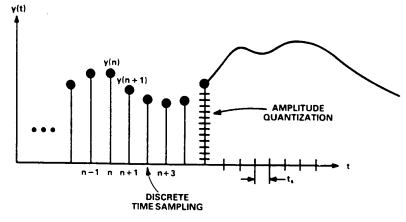
\includegraphics[width=100mm]{./Figures/muestreo1.png}
	\caption{Muestreo discreto de una señal analogica.}
	\label{fig:muestreo1}
\end{figure}

Criterios de Nyquist
\begin{itemize}
\item Una señal analógica con un ancho de banda de \textit{fa} debe ser muestrado a una tasa de muestreo \textit{fs>2fa} para evitar pérdida de información.
\item Si \textit{fs<2fa} entonces un fenómeno llamado \textit{aliasing} ocurre en el ancho de banda de la señal
\end{itemize}

Con el fin de comprender la implicación del \textit{aliasing} se deben considerar los cuatro casos representados en la figura \ref{fig:muestreo2} de una señal senoidal muestreada en el dominio del tiempo.
En el caso 1 está claro que la cantidad de muestras es adecuada para preservar la información. En el caso 2 solo se realizaron 4 muestras por ciclo, pero aun así es una cantidad adecuada para preservar la información. En el caso 3 se representa un caso de la condición límite ambiguo donde \textit{fs=2fa}. Si la relación entre los puntos muestreados y la señal fuese tal que el muestreo coincidiera con los cruces por cero, toda la información se perdería. En el caso 4 la figura representa la situación donde \textit{fs<2fa} y la información obtenida de las muestras dan como resultado una senoide de frecuencia inferior a \textit{fs/2}, en este caso una frecuencia fuera de banda se entrelazo con ancho de banda de Nyquist. 

\begin{figure}[ht]
	\centering
	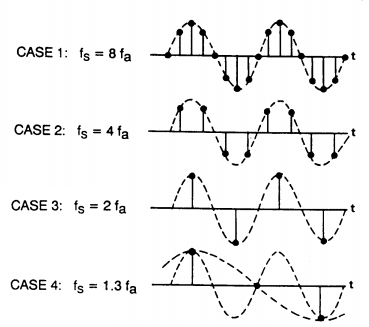
\includegraphics[width=100mm]{./Figures/muestreo2.png}
	\caption{Efecto \textit{aliasing} en señales analogicas.}
	\label{fig:muestreo2}
\end{figure}

Por lo expuesto anteriormente, un conversor analógico digital debe ser precedido por un filtro \textit{anti-aliasing}, figura \ref{fig:muestreo3}, que tenga suficiente atenuación a partir de la frecuencia de corte \textit{fs/2} para prevenir que se entrelacen frecuencias fuera de banda.

\begin{figure}[ht]
	\centering
	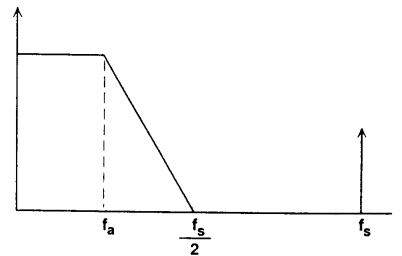
\includegraphics[width=100mm]{./Figures/muestreo3.png}
	\caption{Filtro pasabajos \textit{anti-aliasing}.}
	\label{fig:muestreo3}
\end{figure}

\newpage

\section{Listado de herramientas utilizadas}
Para este trabajo se utilizaron las siguientes herramientas de hardware:
\begin{itemize}
\item Placa LPC Link2 como programador y \textit{debugger}.
\item Placa LPC Link2 como placa de desarrollo.
\item Fuente de alimentación conmutada Minileaf 0-30V 10A
\item Osciloscopio Siglent SDS1202X-E de 200 MHz para verificar las mediciones y tiempos realizados por el equipo.
\item DDS FY6900 de 60 MHz para la generación de señales en el banco de pruebas.
\item Analizador lógico Saleae para el control de tiempos.
\item Multímetro.
\end{itemize}


También se utilizaron las siguientes herramientas de software:
\begin{itemize}
\item Mcuxpresso ide 11.3 para el diseño del firmware \citep{mcuxpresso}.
\item Python 3 para la generación de scripts para el banco de prueba y scripts de procesamiento de datos.
\item Minicom para acceder a la interfaz.
\end{itemize}
